% Options for packages loaded elsewhere
\PassOptionsToPackage{unicode}{hyperref}
\PassOptionsToPackage{hyphens}{url}
%
\documentclass[
]{article}
\usepackage{lmodern}
\usepackage{amssymb,amsmath}
\usepackage{ifxetex,ifluatex}
\ifnum 0\ifxetex 1\fi\ifluatex 1\fi=0 % if pdftex
  \usepackage[T1]{fontenc}
  \usepackage[utf8]{inputenc}
  \usepackage{textcomp} % provide euro and other symbols
\else % if luatex or xetex
  \usepackage{unicode-math}
  \defaultfontfeatures{Scale=MatchLowercase}
  \defaultfontfeatures[\rmfamily]{Ligatures=TeX,Scale=1}
\fi
% Use upquote if available, for straight quotes in verbatim environments
\IfFileExists{upquote.sty}{\usepackage{upquote}}{}
\IfFileExists{microtype.sty}{% use microtype if available
  \usepackage[]{microtype}
  \UseMicrotypeSet[protrusion]{basicmath} % disable protrusion for tt fonts
}{}
\makeatletter
\@ifundefined{KOMAClassName}{% if non-KOMA class
  \IfFileExists{parskip.sty}{%
    \usepackage{parskip}
  }{% else
    \setlength{\parindent}{0pt}
    \setlength{\parskip}{6pt plus 2pt minus 1pt}}
}{% if KOMA class
  \KOMAoptions{parskip=half}}
\makeatother
\usepackage{xcolor}
\IfFileExists{xurl.sty}{\usepackage{xurl}}{} % add URL line breaks if available
\IfFileExists{bookmark.sty}{\usepackage{bookmark}}{\usepackage{hyperref}}
\hypersetup{
  pdftitle={Metatheory.jl: Fast and Elegant Algebraic Computation in Julia with Extensible Equality Saturation},
  hidelinks,
  pdfcreator={LaTeX via pandoc}}
\urlstyle{same} % disable monospaced font for URLs
\usepackage{graphicx}
\makeatletter
\def\maxwidth{\ifdim\Gin@nat@width>\linewidth\linewidth\else\Gin@nat@width\fi}
\def\maxheight{\ifdim\Gin@nat@height>\textheight\textheight\else\Gin@nat@height\fi}
\makeatother
% Scale images if necessary, so that they will not overflow the page
% margins by default, and it is still possible to overwrite the defaults
% using explicit options in \includegraphics[width, height, ...]{}
\setkeys{Gin}{width=\maxwidth,height=\maxheight,keepaspectratio}
% Set default figure placement to htbp
\makeatletter
\def\fps@figure{htbp}
\makeatother
\setlength{\emergencystretch}{3em} % prevent overfull lines
\providecommand{\tightlist}{%
  \setlength{\itemsep}{0pt}\setlength{\parskip}{0pt}}
\setcounter{secnumdepth}{-\maxdimen} % remove section numbering
\ifluatex
  \usepackage{selnolig}  % disable illegal ligatures
\fi
\newlength{\cslhangindent}
\setlength{\cslhangindent}{1.5em}
\newenvironment{cslreferences}%
  {\setlength{\parindent}{0pt}%
  \everypar{\setlength{\hangindent}{\cslhangindent}}\ignorespaces}%
  {\par}

\title{Metatheory.jl: Fast and Elegant Algebraic Computation in Julia
with Extensible Equality Saturation}
\author{}
\date{11 February 2021}

\begin{document}
\maketitle

\hypertarget{summary}{%
\section{Summary}\label{summary}}

The Julia programming language is a fresh approach to technical
computing (Bezanson et al. 2017), disrupting the popular conviction that
a programming language cannot be very high level, easy to learn, and
performant at the same time. One of the most practical features of Julia
is the excellent metaprogramming and macro system, allowing for
programmatic generation and manipulation of Julia expressions as
first-class values in the core language, with a well-known paradigm
similar to LISP idioms such as Scheme, a programming language property
colloquially referred to as \emph{homoiconicity}.

We introduce Metatheory.jl: a general purpose metaprogramming and
algebraic computation library for the Julia programming language,
designed to take advantage of the powerful reflection capabilities to
bridge the gap between symbolic mathematics, abstract interpretation,
equational reasoning, optimization, composable compiler transforms, and
advanced homoiconic pattern matching features. Intuitively,
Metatheory.jl transforms Julia expressions in other Julia expressions
and can achieve such at both compile and run time. This allows
Metatheory.jl users to perform customized and composable compiler
optimization specifically tailored to single, arbitrary Julia packages.
Our library provides a simple, algebraically composable interface to
help scientists in implementing and reasoning about semantics and all
kinds of formal systems, by defining concise rewriting rules in pure,
syntactically valid Julia on a high level of abstraction.

Rewrite rules are defined as regular Julia expressions, manipulating
other syntactically valid Julia expressions: since Julia supports
LaTeX-like abbreviations of UTF8 mathematical symbols as valid operators
and symbols, rewrite theories in Metatheory.jl can bear a strong
structural and visual resemblance to mathematical formalisms encountered
in paper literature.

Theories can then be executed through two, highly composable, rewriting
backends. The first backend relies on a \emph{classic} fixed-point
recursive iteration of AST, with a match-and-replace algorithm built on
top of the (Zhao and Carlsson 2020) pattern matcher. This approach may
be familiar to programmers already experienced in ML-like languages.
This backend is suitable for deterministic recursive algorithms that
intensively use pattern matching on syntax trees, for example, defining
an interpreter from operational or denotational semantics. Nevertheless,
when using this classical approach, even trivial equational rules such
as commutativity and associativity may cause the rewriting algorithm to
loop indefinitely, or to return unexpected results. This is known as
\emph{rewrite order} and is notoriously recognized for requiring
extensive user reasoning about the ordering and structuring of rules to
ensure termination.

\hypertarget{e-graphs-and-equality-saturation}{%
\subsection{E-Graphs and Equality
Saturation}\label{e-graphs-and-equality-saturation}}

This is where the other back-end for Metatheory.jl comes into play. As
the core of our contribution, the equality saturation back-end allows
programmers to define equational theories in pure Julia without worrying
about rule ordering and structuring, by relying on state-of-the-art
techniques for equality saturation over \emph{e-graphs} adapted from the
\texttt{egg} rust library (Willsey et al. 2021). Provided with a theory
of equational rewriting rules, \emph{e-graphs} compactly represent many
equivalent programs. Saturation iteratively executes an e-graph specific
pattern matcher to efficiently compute (and analyze) all possible
equivalent expressions contained in the e-graph congruence closure. This
latter back-end is suitable for partial evaluators, symbolic
mathematics, static analysis, theorem proving and superoptimizers.

\begin{figure}
\centering
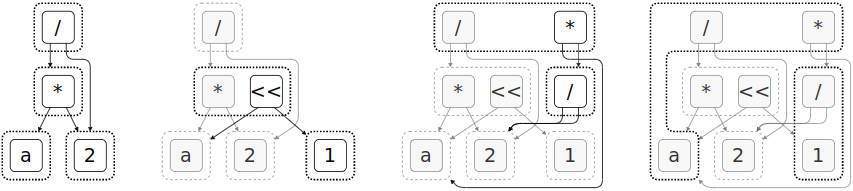
\includegraphics{egraphs.png}
\caption{These four e-graphs represent the process of equality
saturation, adding many equivalent ways to write \((a \times 2) / 2\)
after each iteration. Credits to Max Willsey (Willsey et al.
(2021)).\label{fig:egggg}}
\end{figure}

The original \texttt{egg} library (Willsey et al. 2021) is known to be
the first implementation of generic and extensible e-graphs (Nelson and
Oppen 1980), the contributions of \texttt{egg} include novel amortized
algorithms for fast and efficient equivalence saturation and analysis.
Differently from the original rust implementation of \texttt{egg}, which
handles expressions defined as rust strings and data structures, our
system directly manipulates homoiconic Julia expressions, and can
therefore fully leverage the Julia subtyping mechanism (Zappa Nardelli
et al. 2018), allowing programmers to build expressions containing not
only symbols but all kinds of Julia values. This permits rewriting and
analyses to be efficiently based on runtime data contained in
expressions. Most importantly, users can and are encouraged to include
type assertions in the left hand of rewriting rules in theories.

A project goal of Metatheory, other than being to be easy to use and
composable, is to be fast and efficient: the first-class pattern
matching system and the generation of e-graph analyses from theories
both rely on RuntimeGeneratedFunctions.jl (Rackauckas and Foster 2021),
generating callable functions at runtime that efficiently bypass Julia's
world age problem (Belyakova et al. 2020) with the full performance of a
standard Julia anonymous function.

\hypertarget{analyses-and-extraction}{%
\subsection{Analyses and Extraction}\label{analyses-and-extraction}}

With Metatheory.jl, modeling analyses and conditional/dynamic rewrites
is easy and straightforward: it is possible to check conditions on
runtime values or to read and write from external data structures during
rewriting. The analysis mechanism described in egg and re-implemented in
our contribution lets users define ways to compute additional analysis
metadata from an arbitrary semi-lattice domain, such as costs of nodes
or logical statements attached to terms. Other than for inspection,
analysis data can be used to modify expressions in the e-graph both
during rewriting steps or after e-graph saturation.

Therefore using the equality saturation (e-graph) backend, extraction
can be performed as an on-the-fly e-graph analysis or after saturation.
Users can define their own, or choose between a variety of predefined
cost functions for automatically extracting the most fitting expressions
from the congruence closure represented by an e-graph.

\hypertarget{conclusion}{%
\section{Conclusion}\label{conclusion}}

Many applications of equality saturation have been recently published,
tailoring advanced optimization tasks. Herbie (Panchekha et al. 2015) is
a tool for automatically improving the precision of floating point
expressions, which recently switched to \texttt{egg} as the core
rewriting backend. In (Yang et al., n.d.), authors used \texttt{egg} to
superoptimize tensor signal flow graphs describing neural networks.
However, Herbie requires interoperation and conversion of expressions
between different languages and libraries. Implementing similar case
studies in pure Julia would make valid research contributions on their
own. We are confident that a well-integrated and homoiconic equality
saturation engine in pure Julia will permit exploration of many new
metaprogramming applications, and allow them to be implemented in an
elegant, performant and concise way.

\hypertarget{acknowledgements}{%
\section{Acknowledgements}\label{acknowledgements}}

We acknowledge Max Willsey and contributors for their work on the
original \texttt{egg} library (Willsey et al. 2021), Christopher
Rackauckas and Christopher Foster for their efforts in developing
RuntimeGeneratedFunctions (Rackauckas and Foster 2021), Taine Zhao for
developing MLStyle (Zhao 2021) and MatchCore (Zhao and Carlsson 2020),
and Philip Zucker for his original idea of implementing E-Graphs in
Julia and support during the development of the project.

\hypertarget{references}{%
\section*{References}\label{references}}
\addcontentsline{toc}{section}{References}

\hypertarget{refs}{}
\begin{cslreferences}
\leavevmode\hypertarget{ref-belyakova2020world}{}%
Belyakova, Julia, Benjamin Chung, Jack Gelinas, Jameson Nash, Ross Tate,
and Jan Vitek. 2020. ``World Age in Julia.''

\leavevmode\hypertarget{ref-bezanson2017julia}{}%
Bezanson, Jeff, Alan Edelman, Stefan Karpinski, and Viral B Shah. 2017.
``Julia: A Fresh Approach to Numerical Computing.'' \emph{SIAM Review}
59 (1): 65--98.

\leavevmode\hypertarget{ref-nelson1980fast}{}%
Nelson, Greg, and Derek C Oppen. 1980. ``Fast Decision Procedures Based
on Congruence Closure.'' \emph{Journal of the ACM (JACM)} 27 (2):
356--64.

\leavevmode\hypertarget{ref-panchekha2015automatically}{}%
Panchekha, Pavel, Alex Sanchez-Stern, James R Wilcox, and Zachary
Tatlock. 2015. ``Automatically Improving Accuracy for Floating Point
Expressions.'' \emph{ACM SIGPLAN Notices} 50 (6): 1--11.

\leavevmode\hypertarget{ref-rgf}{}%
Rackauckas, C, and C Foster. 2021. ``RuntimeGeneratedFunctions.jl:
Functions Generated at Runtime Without World-Age Issues.'' \emph{GitHub
Repository}. GitHub.
\url{https://github.com/SciML/RuntimeGeneratedFunctions.jl}.

\leavevmode\hypertarget{ref-egg}{}%
Willsey, Max, Chandrakana Nandi, Yisu Remy Wang, Oliver Flatt, Zachary
Tatlock, and Pavel Panchekha. 2021. ``Egg: Fast and Extensible Equality
Saturation.'' \emph{Proceedings of the ACM on Programming Languages} 5
(POPL): 1--29.

\leavevmode\hypertarget{ref-yang2021equality}{}%
Yang, Yichen, Phitchaya Mangpo Phothilimtha, Yisu Remy Wang, Max
Willsey, Sudip Roy, and Jacques Pienaar. n.d. ``Equality Saturation for
Tensor Graph Superoptimization.'' \emph{arXiv Preprint
arXiv:2101.01332}.

\leavevmode\hypertarget{ref-zappa2018julia}{}%
Zappa Nardelli, Francesco, Julia Belyakova, Artem Pelenitsyn, Benjamin
Chung, Jeff Bezanson, and Jan Vitek. 2018. ``Julia Subtyping: A Rational
Reconstruction.'' \emph{Proceedings of the ACM on Programming Languages}
2 (OOPSLA): 1--27.

\leavevmode\hypertarget{ref-mlstyle}{}%
Zhao, T. 2021. ``MLStyle.jl: Fast, Consistent and Extensible Functional
Programming Infrastructures.'' \emph{GitHub Repository}. GitHub.
\url{https://github.com/thautwarm/MLStyle.jl}.

\leavevmode\hypertarget{ref-matchcore}{}%
Zhao, T, and K Carlsson. 2020. ``MatchCore.jl: A Minimal Implementation
of Optimized Pattern Matching.'' \emph{GitHub Repository}. GitHub.
\url{https://github.com/thautwarm/MatchCore.jl}.
\end{cslreferences}

\end{document}
